

\chapter{Basics}
\label{chapter:basics}
In this background chapter, we review the statistical and probabilistic methodologies .
The goal of this chapter is to provide the basic information regarding Bayesian methods of machine learning used in the thesis. A good introduction to the field can be found in books of \cite{bishop2007pattern}, \cite{kruschke2014doing} and \cite{lee2014bayesian}. The relevant topics from these books are presented below.

\section{Model Based Machine Learning}

Model based machine learning (MBML) is a new paradigm of machine learning, which can be called as the logical convergence between 2 related fields, statistics and machine learning. MBML the goal is to provide a framework which supports the creation of a wide range of models \cite{Bishop20120222}.

In traditional machine learning(SVM, Random Forest etc.) the approach is to map the problem onto a standard algorithm. Thus the algorithm is always fixed and the problem is modified to fit the algorithm.

Model based machine learning has a different take on the problem. Here the approach is to find the model which can represent the problem. The designed model is now used to generate a algorithm which will learn from the data. Thus MBML seeks to create a tailored algorithm for each problem. Such an approach makes the machine learning more flexible and better to understand/explain.

The framework emerged from an important convergence of three key ideas:
   \begin{itemize}
	\item the adoption of Bayesian methodologies for model learning.
	\item the use of graphical models, and
	\item the application of fast, deterministic, efficient and approximate inference algorithms
\end{itemize}

We give a short introduction to Bayesian model learning and graphical models. Inference algorithms is not covered, for a detailed discussion on inference algorithm please refer \cite{beal2003variational}, \cite{minka2001family}

\section{Bayesian Model Learning}

In MBML, models are used to represent the problem. Each problem in machine learning has a two parts: one a set of inputs called observed variables(input features and expected output); second a set of  quantities to be learned called latent unknown variables. In Bayesian modelling both these variables(observed and latent) are probabilities or probability distributions which are updated using Bayes theorem. 

Bayesian models are represented as probability distributions. Probability is used to quantify ``uncertainty" or ``Degree of belief". The models are initialized with some prior probabilities(beliefs). The observed data are used to update the prior beliefs to become posterior beliefs.
\begin{figure}
    \centering
    \begin{subfigure}[b]{0.4\textwidth}
        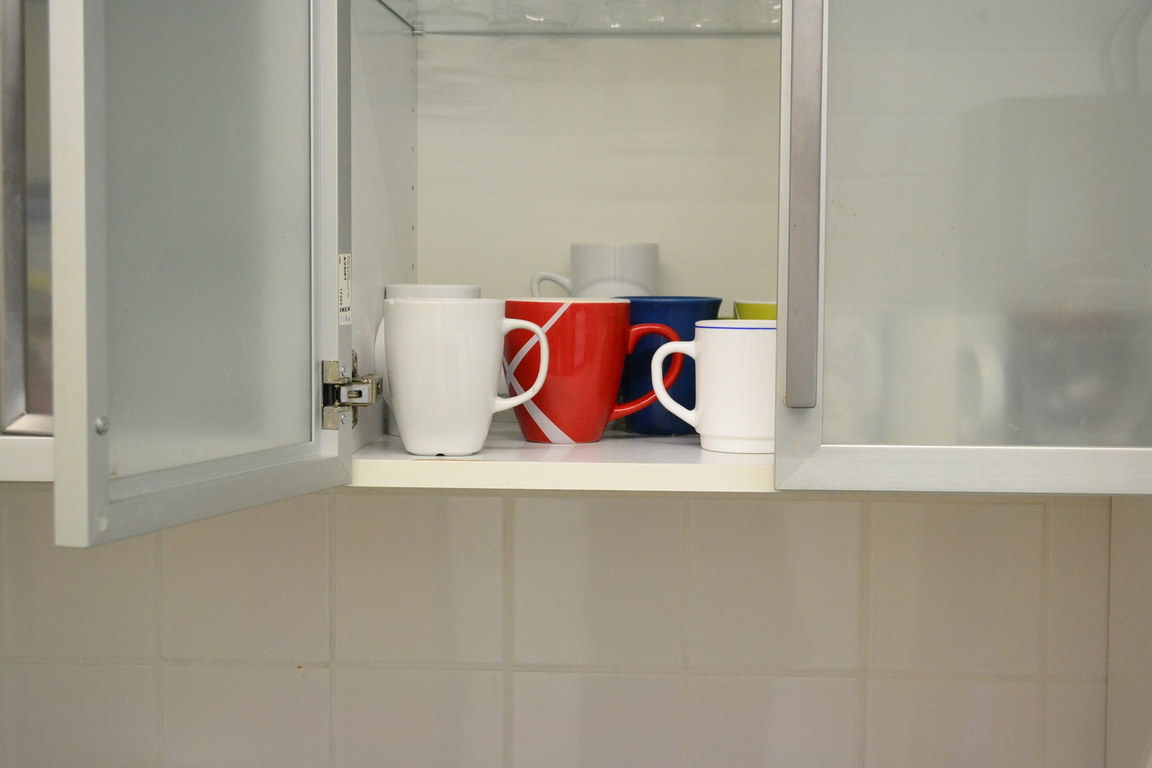
\includegraphics[width=\textwidth]{images/cup_cupboard.jpg}
        \caption{}
        \label{fig:cup-cupboard-basics}
    \end{subfigure}
    ~ %add desired spacing between images, e. g. ~, \quad, \qquad, \hfill etc. 
      %(or a blank line to force the subfigure onto a new line)
      \qquad
    \begin{subfigure}[b]{0.4\textwidth}
        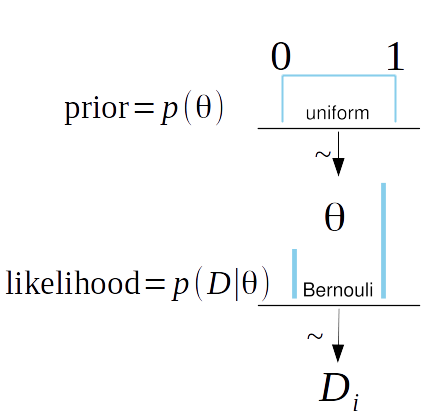
\includegraphics[width=\textwidth]{images/Beta-Bernoulli.png}
        \caption{}
        \label{fig:prior-likelihood}
    \end{subfigure}
\caption[Bayesian learning example]{Bayesian parameter estimation example }
\label{fig: bayes-example}
\end{figure}
We can explain this with an example \cite{lee2014bayesian}. Assume the robot scans a location kitchen cupboard 10 days at 10:00 am and records if it finds a cup. What we want to estimate is the users preference in keeping a cup in the cupboard in morning, which we define as $\theta$, which is the possibility of the user keeping the cup in the cupboard. The directly cannot directly observe the users preference $\theta$. All that it can observe is if the cup is present. Before we do anything else (for example, before we start to look at the data) we need to specify our prior uncertainty with respect to the users preference $\theta$. This uncertainty needs to be expressed as a probability distribution, called the ``prior distribution". In this case, keep in mind that $\theta$ can range from 0 to 1, and that the robot does not know anything about the users behaviour or preferences. Then, a reasonable ``prior distribution,” denoted by $p(\theta)$, is one that assigns equal probability to every value of $\theta$. This uniform distribution is shown by the dotted horizontal line in Figure \ref{fig: bayes}.


\begin{figure}[htp]
\centering

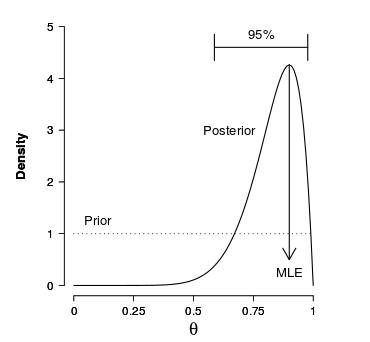
\includegraphics[width=0.5\textwidth]{images/bayes.png}
\caption[Bayesian parameter estimation]{Bayesian parameter estimation for rate parameter $\theta$
, after observing that the cup was present in the cupboard 9 out of 10 days observed. The mode of the posterior distribution for $\theta$ is 0.9, equal to the maximum likelihood estimate (MLE), and the 95\% credible interval extends from 0.59 to 0.98}
\label{fig: bayes}
\end{figure}

Now we consider the observations made by the robot, and find that the cup was present 9 out of 10 days. After observing the data, the updated knowledge about $\theta$ is described by a \emph{posterior distribution}, denoted by $p(\theta | D)$. This distribution expresses the uncertainty about the value of $\theta$, quantifying the relative probability that each possible value is the true value.. Bayes rule specifies how we can combine the information from the data, that is how to determine the posterior distribution $p (\theta | D)$ using  the prior distribution $p(\theta)$ and the likelihood  $p (D | \theta)$ :
\begin{equation}
	p(\theta | D) = \frac{p(D | \theta) p(\theta)}{p(D)}
\end{equation}

The equation is often verbalized as :
\begin{equation}
	posterior = \frac{likelihood * prior}{marginal likelihood}
\end{equation}

We note here that the posterior distribution is a combination of the prior information we had and what we have learned from the data. 




The solid line in Figure ~\ref{fig: bayes} shows the posterior distribution for $\theta$, obtained when the uniform prior is updated with the data. For the posterior distribution in Figure ~\ref{fig: bayes} , a 95\% Bayesian credible interval for $\theta$ extends from 0.59 to 0.98.


\section{Distributions }

The basic idea of Bayesian analysis is that quantifying the \emph{state of belief} or the \emph{state of uncertainty}, about the variables of interest. These variable(latent and observed) are always represented by probability distributions.  Probability distribution is just another name for a probability measure.  In this thesis we exhaustively use the Dirichlet, Categorical and Bernoulli distributions. 
 

\subsection*{Bernoulli distribution}
\todo[inline]{Explain}
Bernoulli distribution is used when there are a number of iterations of some activity, where each iteration (or observation) may turn out to be a ``success" or a ``failure". A Bernoulli distribution takes a single parameter $\theta$, which describes the probability of ``success".  The shorthand $X \sim {\rm Bernoulli}(\theta)$ is used to indicate that the random variable~$X$ has the Bernoulli distribution with parameter~$\theta$, where $0 < \theta < 1$.

A Bernoulli random variable~$X$ with success probability $\theta$ has
probability mass function 
$$
p(x | \theta) = \theta ^ {x} (1 - \theta) ^ {1 - x} \qquad \qquad x = 0, 1
$$
for $0 < \theta < 1$. Figure~\ref{fig:bernoulli_sample} shows 3 Bernoulli distributions with different values of $\theta$.
\begin{figure}[htp]
\centering
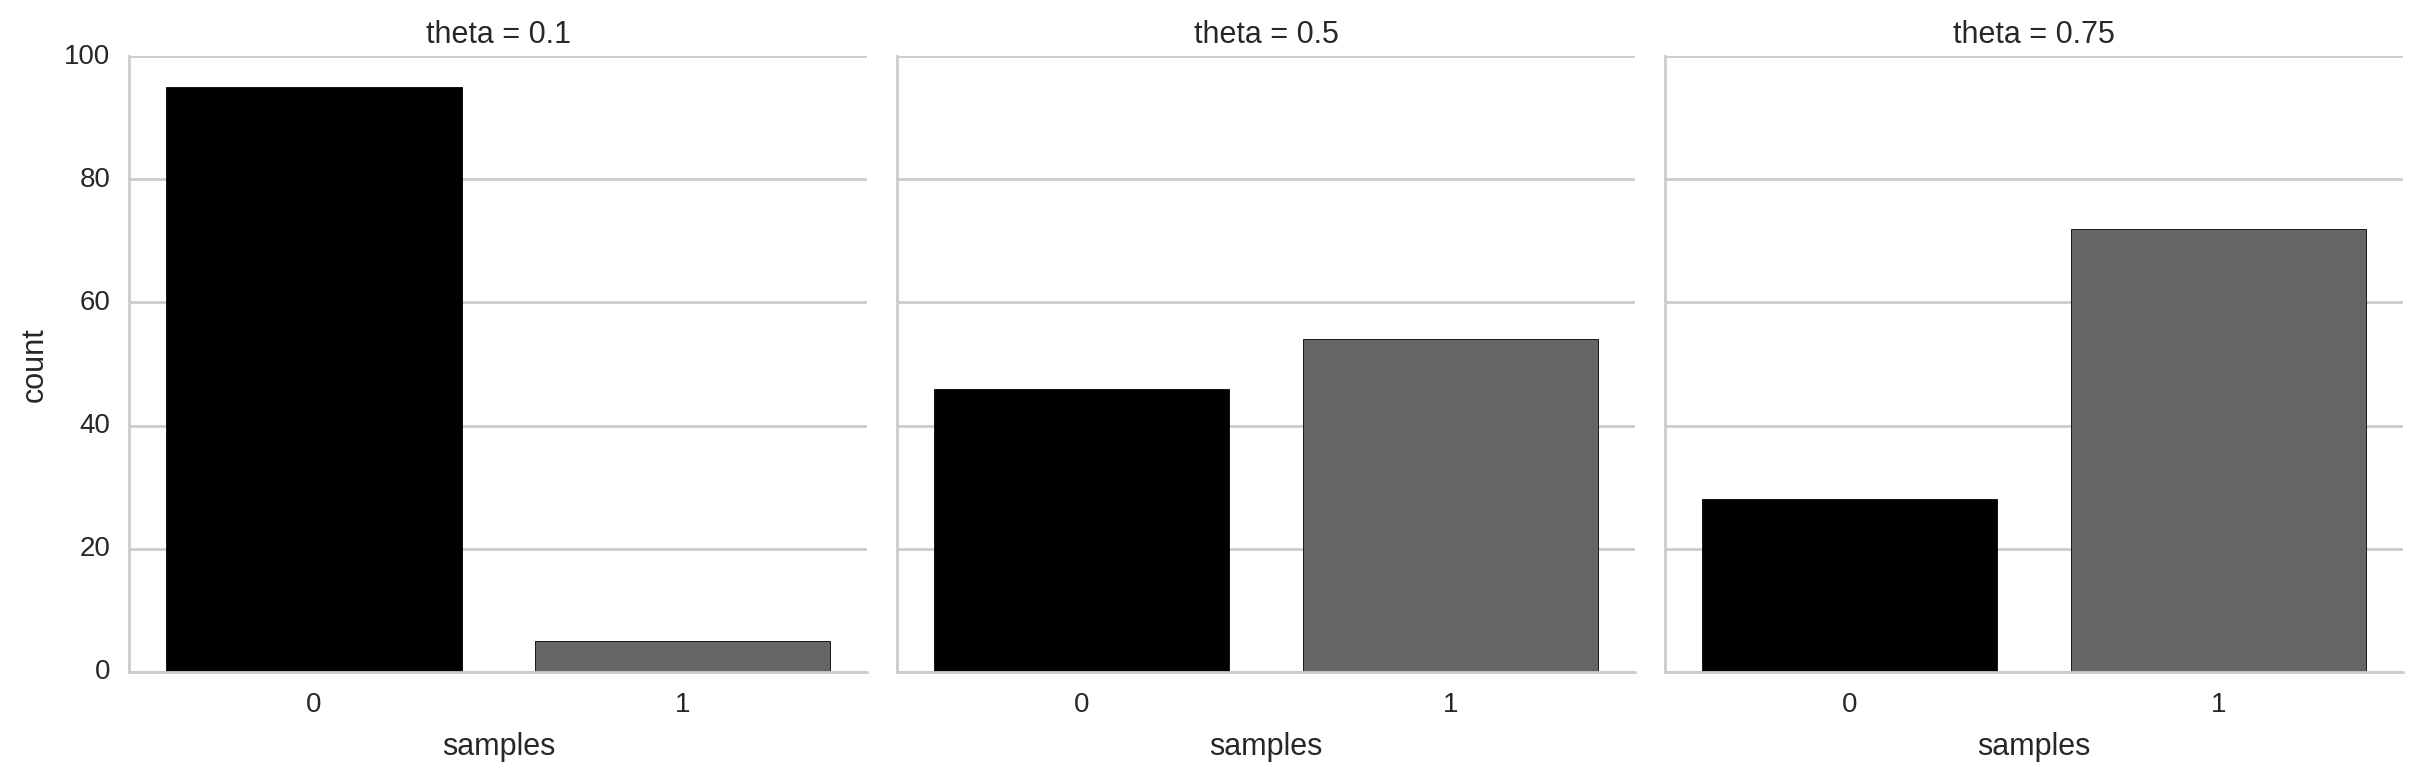
\includegraphics[width=\textwidth]{images/Bernoulli.png}
\caption{Bernoulli Distribution}
\label{fig:bernoulli_sample}
\end{figure}



\subsection*{Categorical distribution}
Categorical distribution is the generalization of the Bernoulli distribution , with more than 2 outcomes.  Categorical takes a parameter $\theta$, which has length k. The probability mass function is :

$$
\prod_{i=1}^k \theta_i^{x_i}
$$

where $\theta_i$ represents the probability of seeing element $i$ and $\sum_{i}p_i = 1$ . This is the formulation adopted by \cite{bishop2007pattern}.  Figure~\ref{fig:Categorical_sample} shows 3 Categorical distributions with different values of $\theta$.

\subsection*{Categorical distribution}
Categorical distribution is the generalization of the Bernoulli distribution , with more than 2 outcomes.  Categorical takes a parameter $\theta$, which has length k. The probability mass function is :

$$
\prod_{i=1}^k \theta_i^{x_i}
$$

where $\theta_i$ represents the probability of seeing element $i$ and $\sum_{i}p_i = 1$ . This is the formulation adopted by \cite{bishop2007pattern}.  Figure~\ref{fig:Categorical_sample} shows 3 Categorical distributions with different values of $\theta$.

\begin{figure}[htp]
\centering
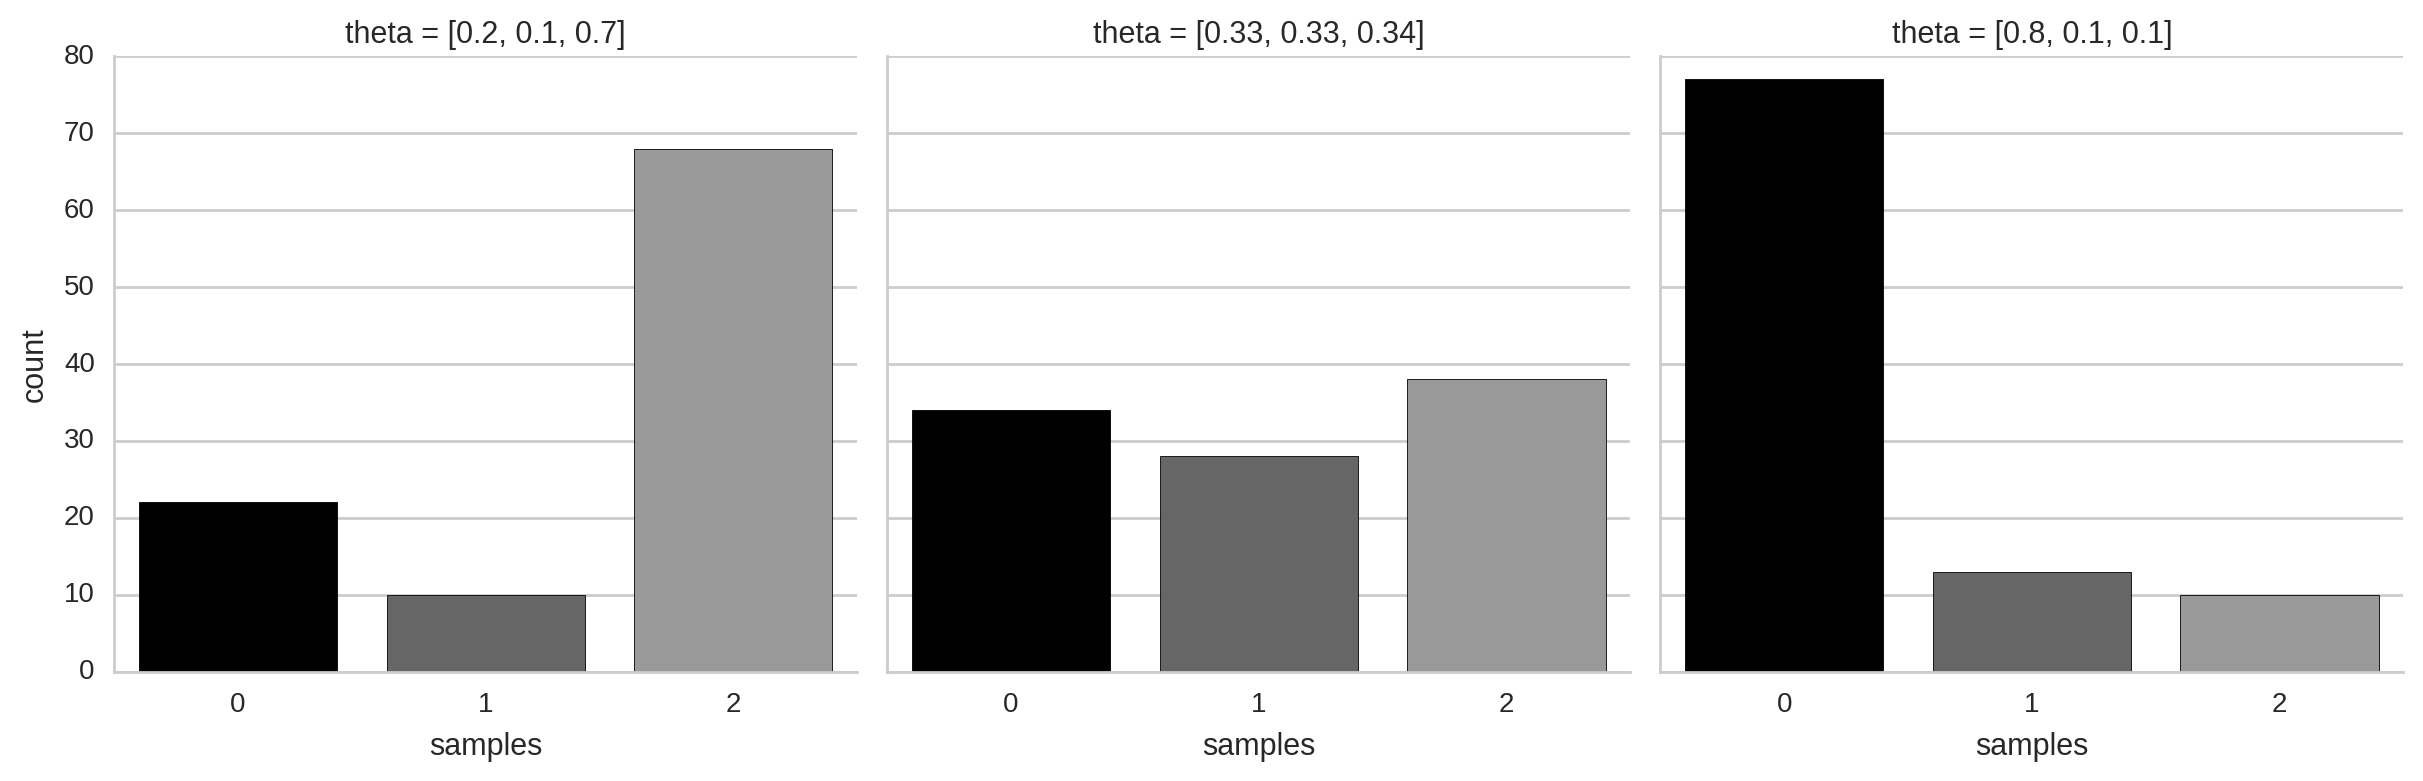
\includegraphics[width=\textwidth]{images/Categorical.png}
\caption{Categorical Distribution}
\label{fig:Categorical_sample}
\end{figure}


\subsection*{Conjugate distribution}
The term conjugate distribution \cite{BS:BS3830070108} refers to cases where the posterior distribution is in the same family as the prior distribution. In Bayesian probability theory, if the posterior distributions $f(\theta | x)$ are in the same family as the prior distributions $f(\theta)$ for all $\theta \in \omega $ the prior and posterior are called conjugate distributions, and the prior is called a conjugate prior. 


\subsection*{Beta distribution}
The beta distribution beta( a, b) is a two-parameter distribution with range [0 , 1] and pdf

\begin{equation}
	p(\theta | a,b) = \frac{(a + b - 1)! }{(a -1 )!(b - 1)!}\theta^{a -1} (1 - \theta)^{b - 1}
\end{equation}

Beta distribution is conjugate prior of Bernoulli and Binomial distributions. Figure~\ref{fig:beta} show Beta distribution with different $a,b$ values.

\begin{figure}[htp]
\centering
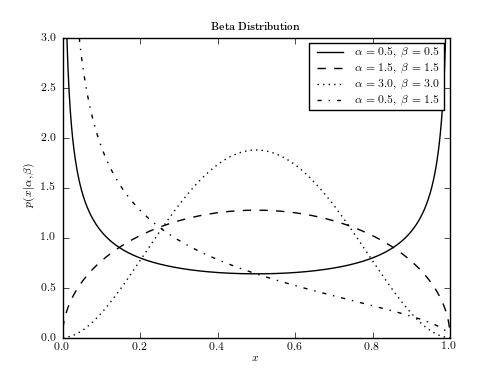
\includegraphics[width=0.5\textwidth]{images/fig_beta_distribution_1.png}
\caption{Beta distribution. \cite{astroMLText}}
\label{fig:beta}
\end{figure}



\subsection*{Dirichlet distribution}
The Dirichlet distribution is part of the exponential family. It has finite dimensional sufficient statistics. It is conjugate to the multinomial and categorical distribution. 


\begin{align*}
    P(\theta) &= \frac{\Gamma(\sum_{k=1}^K \alpha_k)}{\prod_{k=1}^K \Gamma(\alpha_k)}\prod_{k=1}^K \theta_k^{\alpha_k-1} \\
			  &= \frac{1}{Z} \prod_{k=1}^K \theta_k^{\alpha_k-1}
\end{align*}

This is also written as $P(\theta;\alpha)$, $P_\alpha(\theta)$, or $P(\theta|\alpha)$. $\alpha$ is a vector with the same size as $\theta$, and it is known as a ``hyperparameter''.  The choice of $\alpha$ determines the shape of $\theta$'s distribution, which you can see by varying it.  If $\alpha$ is simply a vector of ones, we just get a uniform distribution; all $\theta$s are equally probable.

The below table summarizes which distribution to use and what are their conjugate priors.

\begin{tabular}{|c|c|c|}
\hline
	\textbf{Data type} & \textbf{Distribution} & \textbf{Conjugate prior} \\
\hline
\hline
	Boolean & Bernoulli & Beta \\
\hline
	Ordinal & Binomial & Beta \\
\hline
	Nominal & Categorical , Multinomial & Dirihclet \\
\hline

\end{tabular}


\section{Probabilistic Graphical Models}

Probabilistic Graphical Models (PGM) is the formal lingua franca for probabilistic Bayesian modelling. PGM is a method to visualize complete and interpretable representation of a Bayesian probabilistic model. The nodes in the graph represent variables of the problem, and the edges connecting them represents dependencies. The graph structure is used to indicate dependencies between the variables, with children depending on their parents. The plates are used to indicate replication. We use the conventions of representing unobserved variables without shading and observed variables with shading.

Lets draw the PGM for the problem defined above. Beta distribution with parameters (1,1) can be selected as the prior distribution, while the ability can be represented using Bernoulli distribution. 
The model definition and graphical model are depicted in Figure ~\ref{fig:pgm}

\noindent
\begin{figure}[htp]

\begin{minipage}{0.3\textwidth}
\centering
\tikz {
\centering
 % Define nodes
  \node[latent]                                 (theta) {$\theta$};
  \node[obs, below=of theta]                    (D)     {$D$}; 
  % Connect the nodes
  \edge {theta} {D};
  % plates
  \plate {location} {(D)} {n=0,....,9};
}
\end{minipage}%
\begin{minipage}{0.7\textwidth}
\begin{equation*}
	\theta \sim Beta(1,1) 
\end{equation*}
\begin{equation*}
	P(D|\theta) \sim Bernoulli(\theta)
\end{equation*}
\end{minipage}
\caption[Graphical Model]{Graphical Model: Shaded node observed variable and non-shaded node is latent variable}
\label{fig:pgm}
\end{figure}

\section{Probabilistic Programming Languages}

Probabilistic programming languages(PPL) are new languages developed to program probabilistic graphical models and to run inference in them. Until recently, Bayesian Model learning have been limited in scope, and have been hard to apply to many real-world applications. Probabilistic programming is a new approach using which one can construct Bayesian models faster and in a less error-prone way. 


\begin{figure}[htp]
\centering
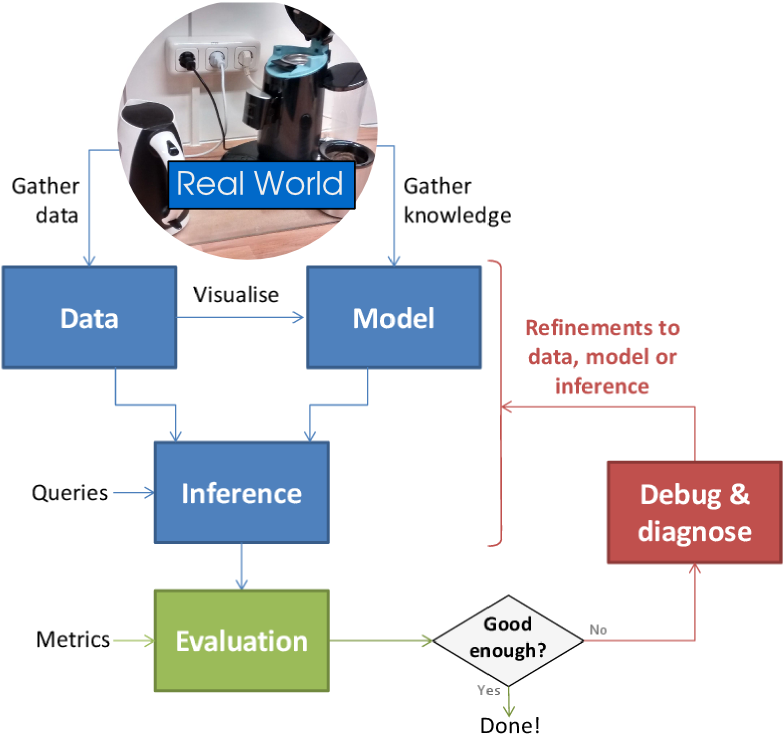
\includegraphics[width=0.5\textwidth]{pictures/Lifecycle.png}
\caption[Steps involved in probabilistic modelling ]{Steps involved in probabilistic modelling  \protect\footnotemark }
\label{}
\end{figure}

\footnotetext{\url{ http://www.mbmlbook.com/LifeCycle.html}}
\textbf{Probabilistic Programming} gives us a framework in which we can create any model, based on our assumptions of the process. The model is basically expressing the assumptions in a mathematical form. The assumptions are the number of variables in the model, the relation between these variables, changes in which variables affects which other variables. This model is then used to generate a problem specific algorithm which can be used to solve the machine learning problem in hand. 

\subsection*{Steps required in Probabilistic Modelling}
\label{sub:steps}
\begin{enumerate}
	\item \textbf{Gather data} to be used for training and evaluation.
    \item \textbf{Gather knowledge} required for model building.
    \item \textbf{Visualise} the data to understand it. This is useful also for gathering knowledge. After visualization the insight gained can be used for assumptions in model building.
    \item \textbf{Construct a model} based on the knowledge of the problem statement available and data visualization. 
    \item \textbf{Perform inference} using both the data and the constructed model. The variables of the model are tuned based on the data available. Predictions can be made to find out the knowledge gained by the model.
    \item \textbf{Evaluate} the performance of the model based on evaluation metric.
    \item \textbf{Diagnose} the model and the assumptions if the evaluation is below some acceptable range
    \item \textbf{Refine the system} by adapting different model structure, inference engine

\end{enumerate}
% subsection steps (end)

Examples of Probabilistic programming languages include CHURCH \cite{goodman_church_2012}, Venture \cite{mansinghka_venture_2014}, PyMC3 \cite{salvatier_probabilistic_2015}, BayesPy \cite{luttinen_bayespy_2014} and Infer.net \cite{minka_2010}. There are many other languages currently in development, and probabilistic programming has become a very active field of research.

\subsection{PyMC3}

\textbf{PyMC3} is python module for Bayesian modelling. It provides intuitive model specification syntax for designing the models. The inference is primarily focussed on advanced Markov chain Monto Carlo fitting algorithms.


\subsection{BayesPy}

\textbf{BayesPy} provides tools to do Bayesian modelling. In BayesPy users construct their models, observes data and then runs inference. The inference engine present in BayesPy is variational Bayesian inference.

Below we show example code of the above explained Beta-Bernoulli model implemented in Bayespy and PyMC3 .

\noindent\begin{minipage}{.46\textwidth}
\begin{lstlisting}[caption=BayesPy Code,frame=tlrb]{Name}
import bayespy as bp

observations = [1, 1, 1, 1, 0, 1, 1, 1, 1, 1]


theta = bp.Beta([1, 1])
D = bp.Bernoulli(theta, plates=(10,))
D.observe(observations)
theta.update()

\end{lstlisting}
\end{minipage}\hfill
\begin{minipage}{.46\textwidth}
\begin{lstlisting}[caption=PyMC3 code,frame=tlrb]{Name}
import pymc3 as pm

observations = [1, 1, 1, 1, 0, 1, 1, 1, 1, 1]

with pm.Model() as model:
    theta = pm.Beta(1, 1)
    D = pm.Bernoulli(observed=observations)
    step = pm.NUTS() 
    trace = pm.sample(100, step)
    
\end{lstlisting}

\end{minipage}


Thus the same graphical model is implemented in two different languages. The user doesn't need to worry about the underlying distribution implementations an work directly at the model level. This makes modelling easy and less error-prone. 